% chktex-file 3
% chktex-file 8
% chktex-file 10
% chktex-file 13
% chktex-file 17
% chktex-file 24
% chktex-file 25
% chktex-file 36
% chktex-file 37

%%%%%%%%%%%%%%%%%%%%%%%%%%%%%%%%%%%%%%%%%%%%%%%%%%%%%%%%%%%%%%%%%%%%%%%%%%%%%%%%%%%%%%%%%%%%%%%%%%%%%%%%%%%%%%%%%%%%%%%%

\chapter{Four-digit NACA Airfoil}
% ref: https://en.wikipedia.org/wiki/NACA_airfoil#Five-digit_series

%%%%%%%%%%%%%%%%%%%%%%%%%%%%%%%%%%%%%%%%%%%%%%%%%%%%%%%%%%%%%%%%%%%%%%%%%%%%%%%%%%%%%%%%%%%%%%%%%%%%%%%%%%%%%%%%%%%%%%%%

Terminology used for defining the airfoil:
\begin{enumerate}
    \item
    Chord ($c$)
    \item
    Maximum camber ($m$)
    \item
    Maximum camber location ($p$)
    \item
    Maximum thickness ($h$)
    \item
    Camber line (red dashed line)
    \item
    Leading edge ($x=0, y=0$)
    \item
    Trailing edge ($x=c, y=0$)
\end{enumerate}
\begin{figure}[h!]
    \centering
    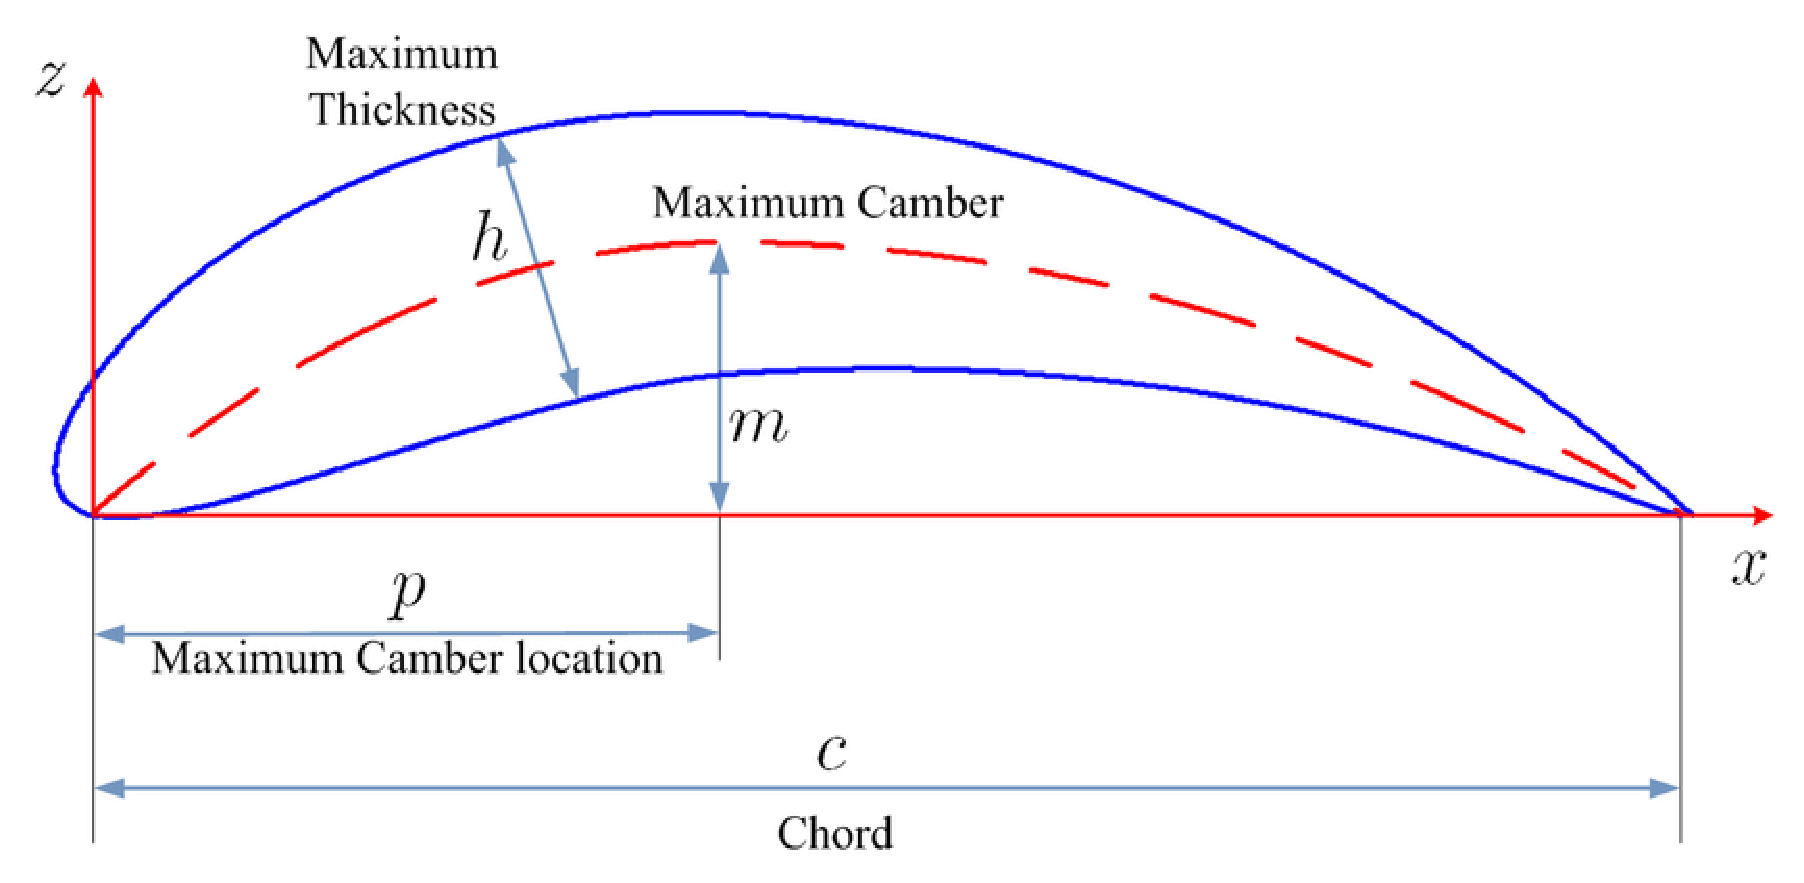
\includegraphics[width=0.5\textwidth]{airfoil_shape_image.eps}
    \caption{The parameters in wing profile.}
    \label{f:airfoil_shape_image}
\end{figure}
% figure downloaded from: https://www.researchgate.net/figure/AIRFOIL-SHAPE-PARAMETERS_fig4_267490031

The wing profile is defined by four-digit ($\mathrm{XYZZ}$):
\begin{enumerate}
    \item
    The 1st digit is the maximum camber as percentage of the chord.
    \begin{equation*}
        m = c \times (\mathrm{X}/100)
    \end{equation*}
    \item
    The 2nd digit is the maximum camber location in tenths of the chord.
    \begin{equation*}
        p = c \times (\mathrm{Y}/10)
    \end{equation*}
    \item
    The last two digits are the maximum thickness as percent of the chord.
    \begin{equation*}
        h = c \times (\mathrm{ZZ}/100)
    \end{equation*}
\end{enumerate}

The formula to calculate the thickness is
\begin{equation*}
    y_h = 5h\left( 0.2969\sqrt{x}-0.1260x-0.3516x^2+0.2843x^3-0.1015x^4 \right)
\end{equation*}
where $x$ is the position along the chord (from $0$ to $1$), $y_h$ is the half thickness at a given value of $x$, and
$h$ is the maximum thickness.

The camber line equation is
\begin{equation*}
    y_c =
    \begin{cases}
    \frac{m}{p^2} (2px-x^2); & 0 \leq x \leq p \\
    \frac{m}{(1-p)^2} (1-2p+2px-x^2);  &  p \leq x \leq 1
    \end{cases}
\end{equation*}
where $y_c$ is the camber line point at a given value of $x$, $m$ is the maximum camber, and $p$ is the location of
maximum camber.

The point $\mathbf{F}_u(x)$ in upper surface equation is
\begin{equation}
    \mathbf{F}_u(x) =
    \begin{bmatrix}
        x_u \\ y_u
    \end{bmatrix}
    =
    \begin{bmatrix}
        x - y_h \sin\theta \\ y_c + y_h \cos\theta
    \end{bmatrix}
    \label{e:naca:up_xy}
\end{equation}
and the point $\mathbf{F}_l(x)$ in lower surface equation is
\begin{equation*}
    \mathbf{F}_l(x) =
    \begin{bmatrix}
        x_u \\ y_u
    \end{bmatrix}
    =
    \begin{bmatrix}
        x + y_h \sin\theta \\ y_c - y_h \cos\theta
    \end{bmatrix}
\end{equation*}
where
\begin{equation*}
    \arctan \theta =
    \begin{cases}
    \frac{2m}{p^2} (p-x); & 0 \leq x \leq p \\
    \frac{2m}{(1-p)^2} (p-x);  &  p \leq x \leq 1
    \end{cases}
\end{equation*}